\section{Subsistema de Visión: Hardware y Soporte}

El subsistema de visión constituye el sensor primario del kit, proporcionando información visual del espacio de trabajo para la detección, localización y clasificación de objetos. La selección del hardware de captura de imágenes debe equilibrar capacidad de percepción, compatibilidad de software, costo y complejidad de integración.

\subsection{Requerimientos del Sistema de Visión}

Para definir las especificaciones de la cámara, se identificaron los siguientes requerimientos funcionales y técnicos:

\subsubsection{Requerimientos Funcionales}

\begin{itemize}
    \item Detección de objetos de dimensiones conocidas (25 mm × 25 mm) sobre superficie plana
    \item Segmentación por color de objetos sobre fondo blanco (zona de recolección) o negro (plataforma base)
    \item Determinación de posición 2D (coordenadas x, y) de objetos en el plano de trabajo
    \item Frecuencia de captura: 10-15 fps mínimo para operación en tiempo real
    \item Resolución suficiente para distinguir objetos separados por 10 mm mínimo
\end{itemize}

\subsubsection{Requerimientos Técnicos}

\begin{itemize}
    \item Compatibilidad nativa con Ubuntu 24.04 LTS
    \item Integración con ROS2 Jazzy Jalisco mediante nodos estándar
    \item Interfaz USB para conexión directa a Raspberry Pi 5
    \item Configuración automática sin drivers propietarios
    \item Campo de visión adecuado para capturar área de trabajo de 550 mm × 360 mm desde altura de montaje
    \item Iluminación: Funcionamiento bajo iluminación artificial de laboratorio (400-600 lux)
\end{itemize}

\subsubsection{Restricciones del Proyecto}

\begin{itemize}
    \item Presupuesto máximo por cámara: 150,000 COP
    \item Peso y dimensiones compatibles con soporte estructural en FDM
    \item Disponibilidad comercial en mercado nacional
    \item Documentación y soporte comunitario disponible
\end{itemize}

\subsection{Cámaras Evaluadas}

Se evaluaron tres cámaras con diferentes capacidades de percepción y rangos de precio:

\subsubsection{ORBBEC Astra Pro}

Cámara de profundidad RGB-D diseñada para aplicaciones de robótica y reconocimiento de gestos. Especificaciones principales \cite{Orbbec2024AstraPro}:

\begin{itemize}
    \item Tecnología: Sensor RGB + sensor de profundidad por luz estructurada
    \item Rango de operación: 0.6-8.0 m
    \item Resolución RGB: 640 × 480 @ 30 fps
    \item Resolución de profundidad: 640 × 480 @ 30 fps
    \item Campo de visión: 60° H × 49.5° V (RGB), 60° H × 45° V (profundidad)
    \item Interfaz: USB 2.0
    \item Dimensiones: 165 mm × 40 mm × 30 mm
    \item Peso: 310 g
    \item Costo: 340,000 COP
\end{itemize}

\paragraph{Ventajas}
\begin{itemize}
    \item Generación de mapas de puntos 3D (point clouds) para reconstrucción de escena
    \item Datos de profundidad permiten algoritmos de agarre más sofisticados
    \item Adecuada para aplicaciones de navegación y mapeo SLAM
\end{itemize}

\paragraph{Desventajas}
\begin{itemize}
    \item Requiere drivers propietarios provistos por ORBBEC
    \item Compatibilidad limitada: ROS2 Humble, sin soporte oficial para ROS2 Jazzy
    \item Costo elevado (3.2 veces el presupuesto objetivo)
    \item Mayor peso y dimensiones complican el diseño del soporte
    \item Complejidad de calibración y configuración
\end{itemize}

\subsubsection{ORBBEC Astra Somatosensorial}

Versión económica de cámara de profundidad para aplicaciones de realidad virtual y reconocimiento de gestos \cite{Orbbec2024Astra}:

\begin{itemize}
    \item Tecnología: Sensor RGB + profundidad por luz estructurada
    \item Rango de operación: 0.6-8.0 m
    \item Resolución RGB: 640 × 480 @ 30 fps
    \item Resolución de profundidad: 320 × 240 @ 30 fps
    \item Interfaz: USB 2.0
    \item Costo: 180,000 COP
\end{itemize}

\paragraph{Ventajas}
\begin{itemize}
    \item Capacidad de generación de mapas de puntos y profundidad
    \item Costo intermedio entre opciones evaluadas
\end{itemize}

\paragraph{Desventajas}
\begin{itemize}
    \item Drivers propietarios requeridos
    \item Compatibilidad limitada: ROS1 Noetic únicamente, sin soporte para ROS2
    \item Obsolescencia: ROS1 alcanzó fin de vida en mayo de 2025 \cite{ROS2EOL2024}
    \item Resolución de profundidad reducida (320 × 240) limita precisión
\end{itemize}

\subsubsection{Logitech C270 HD Webcam}

Cámara web de consumo con amplia compatibilidad en sistemas Linux \cite{Logitech2024C270}:

\begin{itemize}
    \item Tecnología: Sensor CMOS RGB convencional
    \item Resolución: 1280 × 720 @ 30 fps (HD), 640 × 480 @ 30 fps (VGA)
    \item Campo de visión: 60° diagonal
    \item Enfoque: Fijo
    \item Interfaz: USB 2.0 (UVC - USB Video Class)
    \item Dimensiones: 70 mm × 32 mm × 60 mm
    \item Peso: 75 g
    \item Costo: 106,000 COP
\end{itemize}

\paragraph{Ventajas}
\begin{itemize}
    \item Compatibilidad nativa con Ubuntu 24.04 LTS mediante drivers UVC del kernel Linux
    \item Integración directa con ROS2 Jazzy mediante paquetes estándar (usb\_cam, v4l2\_camera) \cite{ROS2Camera2024}
    \item No requiere drivers propietarios ni compilación de software adicional
    \item Costo dentro del presupuesto objetivo (71\% del límite)
    \item Peso ligero (75 g) simplifica diseño de soporte
    \item Dimensiones compactas facilitan integración
    \item Amplia documentación y soporte comunitario
    \item Disponibilidad comercial inmediata en mercado nacional
\end{itemize}

\paragraph{Desventajas}
\begin{itemize}
    \item No proporciona información de profundidad
    \item Sensor 2D limita aplicaciones de reconstrucción 3D
    \item Calidad de imagen inferior a cámaras industriales
    \item Enfoque fijo puede requerir ajuste de distancia de montaje
\end{itemize}

\subsection{Análisis Comparativo}

La Tabla \ref{tab:comparacion_camaras} presenta una comparación sistemática de las especificaciones técnicas y características operativas de las tres cámaras evaluadas.

\begin{table}[H]
\centering
\caption{Comparación de especificaciones de cámaras evaluadas}
\label{tab:comparacion_camaras}
\small
\begin{tabular}{|l|l|l|l|}
\hline
\textbf{Característica} & \textbf{Astra Pro} & \textbf{Astra Soma.} & \textbf{Logitech C270} \\
\hline
Tipo de sensor & RGB-D & RGB-D & RGB \\
Resolución RGB & 640×480 & 640×480 & 1280×720 \\
Profundidad & Sí (640×480) & Sí (320×240) & No \\
Frame rate & 30 fps & 30 fps & 30 fps \\
Interfaz & USB 2.0 & USB 2.0 & USB 2.0 (UVC) \\
Peso & 310 g & ~250 g & 75 g \\
Drivers & Propietarios & Propietarios & UVC nativo \\
Ubuntu 24.04 & Limitado & No & Nativo \\
ROS2 Jazzy & No oficial & No & Nativo \\
ROS1 Noetic & Sí & Sí & Sí \\
Costo (COP) & 340,000 & 180,000 & 106,000 \\
Disponibilidad & Importación & Importación & Nacional \\
\hline
\end{tabular}
\end{table}

\subsection{Matriz de Decisión}

Para evaluar objetivamente las alternativas, se desarrolló una matriz de decisión multicriterio ponderada (Tabla \ref{tab:matriz_decision_camara}). Los criterios se ponderaron según su importancia relativa para los objetivos del proyecto educativo.

\begin{table}[H]
\centering
\caption{Matriz de decisión para selección de cámara}
\label{tab:matriz_decision_camara}
\small
\begin{tabular}{|l|c|c|c|c|c|c|c|}
\hline
\textbf{Criterio} & \textbf{Peso} & \multicolumn{2}{c|}{\textbf{Astra Pro}} & \multicolumn{2}{c|}{\textbf{Astra Soma.}} & \multicolumn{2}{c|}{\textbf{C270}} \\
 & (\%) & Calif. & Pond. & Calif. & Pond. & Calif. & Pond. \\
\hline
Compatibilidad SW & 25 & 5 & 1.25 & 3 & 0.75 & 10 & 2.50 \\
Costo & 20 & 3 & 0.60 & 6 & 1.20 & 9 & 1.80 \\
Facilidad integración & 20 & 4 & 0.80 & 4 & 0.80 & 10 & 2.00 \\
Disponibilidad & 15 & 5 & 0.75 & 5 & 0.75 & 10 & 1.50 \\
Capacidad percepción & 10 & 10 & 1.00 & 8 & 0.80 & 6 & 0.60 \\
Peso/dimensiones & 5 & 5 & 0.25 & 6 & 0.30 & 10 & 0.50 \\
Documentación & 5 & 6 & 0.30 & 5 & 0.25 & 10 & 0.50 \\
\hline
\textbf{TOTAL} & \textbf{100} & --- & \textbf{4.95} & --- & \textbf{4.85} & --- & \textbf{9.40} \\
\hline
\end{tabular}
\end{table}

\textit{Nota: Calificación en escala de 1 a 10, donde 10 es el mejor desempeño.}

\subsection{Justificación de la Selección}

La Logitech C270 fue seleccionada como cámara del sistema de visión del kit por obtener la puntuación ponderada más alta (9.40) en la matriz de decisión. Las razones técnicas específicas son:

\subsubsection{Compatibilidad de Software}

La compatibilidad nativa con Ubuntu 24.04 LTS y ROS2 Jazzy mediante el estándar UVC (USB Video Class) elimina dependencias de drivers propietarios. Esto garantiza:

\begin{itemize}
    \item Operación inmediata sin compilación de software adicional
    \item Compatibilidad futura con actualizaciones del sistema operativo
    \item Independencia de ciclos de soporte del fabricante
    \item Simplicidad en la configuración por parte de estudiantes
\end{itemize}

El soporte mediante paquetes estándar de ROS2 (usb\_cam, v4l2\_camera, image\_pipeline) permite integración directa con pipelines de procesamiento de imágenes y nodos de visión por computador \cite{ROS2Camera2024}.

\subsubsection{Adecuación a Requerimientos de Percepción}

A pesar de no proporcionar información de profundidad, la C270 es completamente adecuada para los requerimientos específicos del kit:

\begin{enumerate}
    \item \textbf{Escenario estático}: La plataforma base permanece fija durante operación. Las posiciones de zonas de recolección, depósito y base del manipulador son conocidas y constantes. No se requiere reconstrucción 3D dinámica del entorno
    
    \item \textbf{Objetos planares}: Los objetos de clasificación reposan sobre superficies planas (zona de recolección o interior de canecas). Su orientación es predecible (caras superior o inferior hacia arriba)
    
    \item \textbf{Dimensiones conocidas}: Los objetos tienen dimensiones estándar de 25 mm × 25 mm. El tamaño aparente en la imagen permite inferir profundidad relativa mediante geometría proyectiva simple
    
    \item \textbf{Estrategia de agarre}: El sistema de succión por vacío no requiere información precisa de orientación 3D del objeto, solo su posición 2D en el plano de trabajo
    
    \item \textbf{Calibración estática}: La altura de la cámara sobre la plataforma es fija y conocida, permitiendo transformaciones 2D pixel-a-mundo mediante calibración única
\end{enumerate}

Para estas condiciones operativas, la información de profundidad proporcionada por cámaras RGB-D no aporta valor funcional significativo, mientras que incrementa sustancialmente complejidad y costo \cite{Corke2017Robotics}.

\subsubsection{Costo-Efectividad}

El costo de 106,000 COP representa:
\begin{itemize}
    \item 31\% del costo de la Astra Pro (ahorro de 234,000 COP)
    \item 59\% del costo de la Astra Somatosensorial (ahorro de 74,000 COP)
    \item Presupuesto disponible para 7 kits: 742,000 COP vs 2,380,000 COP (Astra Pro)
\end{itemize}

Este ahorro permite asignar recursos a otros componentes del kit o fabricar unidades adicionales.

\subsubsection{Simplicidad de Integración}

La integración plug-and-play elimina barreras técnicas para estudiantes:
\begin{itemize}
    \item No requiere compilación de drivers desde fuente
    \item Configuración mediante archivos launch estándar de ROS2
    \item Troubleshooting simplificado (herramientas estándar de Linux: v4l2-ctl, cheese)
    \item Tiempo de configuración: <5 minutos vs >2 horas para cámaras con drivers propietarios
\end{itemize}

\subsubsection{Factor de Forma}

El peso de 75 g y dimensiones compactas (70 mm × 32 mm × 60 mm) simplifican el diseño del soporte:
\begin{itemize}
    \item Menor carga sobre estructura en FDM (reducción de deflexión)
    \item Posibilidad de montaje en configuraciones alternativas
    \item Menor inercia durante ajustes de posición
\end{itemize}

\subsection{Consideraciones sobre Profundidad en Robótica Educativa}

Es importante contextualizar la decisión de prescindir de sensores de profundidad. Si bien las cámaras RGB-D son herramientas poderosas en robótica avanzada (navegación autónoma, SLAM, agarre de objetos desconocidos) \cite{Rosinol2020Kimera}, su utilidad en contextos educativos debe evaluarse críticamente:

\begin{itemize}
    \item \textbf{Complejidad conceptual}: Estudiantes deben dominar primero visión 2D (filtrado, segmentación, morfología) antes de abordar reconstrucción 3D
    
    \item \textbf{Carga computacional}: Procesamiento de point clouds requiere recursos que competirían con otros nodos de ROS2 en la Raspberry Pi 5
    
    \item \textbf{Tiempo de desarrollo}: Algoritmos 3D requieren semanas de desarrollo vs días para visión 2D en entornos estructurados
    
    \item \textbf{Curva de aprendizaje}: Herramientas como PCL (Point Cloud Library) tienen mayor barrera de entrada que OpenCV para visión 2D
\end{itemize}

Para un kit educativo que busca enseñar fundamentos de robótica, visión por computador y ROS2, una cámara 2D bien integrada proporciona mejor balance entre capacidad didáctica y complejidad técnica.

\subsection{Conclusión}

La selección de la Logitech C270 como cámara del kit se fundamenta en su compatibilidad nativa con la pila de software seleccionada (Ubuntu 24.04 + ROS2 Jazzy), su adecuación completa a los requerimientos funcionales de percepción en entorno estructurado, su costo accesible que permite fabricación de múltiples unidades, y su simplicidad de integración que reduce barreras técnicas para estudiantes. La ausencia de información de profundidad no constituye una limitación para las tareas de clasificación en ambiente estático con objetos de dimensiones conocidas.

\subsection{Selección de Tubos para Soporte de Cámara}

El soporte de la cámara debe proporcionar una plataforma estable elevada sobre la plataforma base del kit, garantizando un campo de visión adecuado del área de trabajo. La selección del material estructural para este soporte debe equilibrar rigidez mecánica, peso, disponibilidad comercial y compatibilidad con el espacio designado en el layout.

\subsubsection{Requerimientos del Soporte}

El sistema de soporte de cámara debe cumplir los siguientes requerimientos:

\paragraph{Requerimientos Geométricos}

\begin{itemize}
    \item Altura de montaje: 400-500 mm sobre la plataforma base para campo de visión completo
    \item Restricción de diámetro: Máximo 1 pulgada (25.4 mm) para compatibilidad con espacio designado en layout (Figura \ref{fig:layout2})
    \item Configuración: Estructura vertical con brazo horizontal en voladizo para posicionamiento de cámara sobre centro de zona de trabajo
\end{itemize}

\paragraph{Requerimientos Mecánicos}

\begin{itemize}
    \item Carga: Cámara Logitech C270 (75 g) + soporte impreso en FDM (~50 g) = 125 g total
    \item Deflexión máxima: <5 mm en el extremo del voladizo bajo carga estática
    \item Estabilidad: Resistencia a vibraciones generadas por movimientos del manipulador
    \item Factor de seguridad: Mínimo 3× respecto a carga de operación
\end{itemize}

\paragraph{Requerimientos Operativos}

\begin{itemize}
    \item Facilidad de ajuste: Posibilidad de modificar altura y orientación de cámara sin herramientas especializadas
    \item Accesibilidad: No debe interferir con acceso a zonas de depósito o área de electrónica
    \item Estética: Apariencia profesional apropiada para entorno educativo
    \item Disponibilidad: Material disponible en ferreterías nacionales con accesorios estándar
\end{itemize}

\subsubsection{Materiales Evaluados}

Se evaluaron tres opciones de tubería estructural disponibles comercialmente en el mercado nacional:

\paragraph{Tubo Closet Ovalado de Aluminio Anodizado}

Tubo de perfil ovalado diseñado originalmente para sistemas de closet y organización de ropa \cite{Fixser2024Closet}:

\begin{itemize}
    \item Material: Aleación de aluminio 6063-T5 con anodizado niquelado
    \item Dimensiones: 0.8 mm espesor × 15 mm ancho × 30 mm alto (perfil ovalado)
    \item Longitud comercial: 3 m
    \item Peso lineal: Aproximadamente 0.3 kg/m
    \item Módulo de elasticidad: 69 GPa (aluminio)
    \item Momento de inercia: ~4,500 mm$^4$ (eje mayor)
    \item Acabado: Anodizado niquelado decorativo
    \item Costo: 8,300 COP/m
    \item Fabricante: Fixser
\end{itemize}

\textbf{Ventajas:}
\begin{itemize}
    \item Material liviano (densidad 2.7 g/cm$^3$)
    \item Diseñado específicamente para soportar cargas en voladizo (ropa en percha)
    \item Acabado estético profesional (niquelado)
    \item Perfil ovalado proporciona mayor rigidez en dirección de carga que perfil circular equivalente
    \item Resistencia a corrosión por anodizado
\end{itemize}

\textbf{Desventajas:}
\begin{itemize}
    \item Rigidez inferior al acero (1/3 del módulo de elasticidad)
    \item Accesorios de unión no estándar, requieren diseño personalizado
\end{itemize}

\paragraph{Tubo de PVC Sanitario Grado Presión}

Tubería de PVC (policloruro de vinilo) utilizada en instalaciones hidráulicas \cite{PVC2024Sanitario}:

\begin{itemize}
    \item Material: PVC rígido (Policloruro de vinilo)
    \item Diámetro nominal: 1 pulgada (25.4 mm externo)
    \item Espesor de pared: 2.4 mm (Schedule 40)
    \item Longitud comercial: 3 m
    \item Peso lineal: Aproximadamente 0.4 kg/m
    \item Módulo de elasticidad: 2.4-4.1 GPa (PVC rígido)
    \item Costo: 7,800 COP/m
    \item Disponibilidad de accesorios: Codos, tees, uniones, acoples roscados hembra/macho
\end{itemize}

\textbf{Ventajas:}
\begin{itemize}
    \item Material liviano (densidad 1.4 g/cm$^3$)
    \item Ecosistema completo de accesorios estandarizados (codos 90°, tees, acoples roscados)
    \item Costo más bajo por metro lineal
    \item Facilidad de corte y manipulación sin herramientas especializadas
    \item Resistencia química y a humedad
\end{itemize}

\textbf{Desventajas:}
\begin{itemize}
    \item Módulo de elasticidad muy bajo (2.4-4.1 GPa) resulta en deflexiones significativas
    \item Susceptibilidad a deformación plástica bajo carga sostenida (creep)
    \item Acabado blanco o gris poco estético para aplicación visible
    \item Resistencia reducida a temperaturas elevadas (>60°C)
\end{itemize}

\paragraph{Tubo de Acero Galvanizado Grado Estructural}

Tubería de acero con recubrimiento galvanizado para aplicaciones de cerramiento y estructuras \cite{Acero2024Galvanizado}:

\begin{itemize}
    \item Material: Acero estructural ASTM A53 con galvanizado Z180
    \item Diámetro nominal: 1 pulgada (26.7 mm externo)
    \item Espesor de pared: 1.5 mm
    \item Longitud comercial: 6 m
    \item Peso lineal: Aproximadamente 1.1 kg/m
    \item Módulo de elasticidad: 200 GPa (acero)
    \item Costo: 8,150 COP/m
    \item Disponibilidad de accesorios: Codos, tees, uniones, acoples roscados
\end{itemize}

\textbf{Ventajas:}
\begin{itemize}
    \item Rigidez máxima (módulo de elasticidad 200 GPa)
    \item Deflexión mínima bajo carga (<1 mm para voladizo de 400 mm)
    \item Ecosistema completo de accesorios roscados estándar
    \item Resistencia mecánica superior (límite elástico ~250 MPa)
    \item Durabilidad extendida por galvanizado
\end{itemize}

\textbf{Desventajas:}
\begin{itemize}
    \item Peso elevado (1.1 kg/m, 4× el aluminio)
    \item Acabado galvanizado industrial poco estético
    \item Requiere herramientas para corte (sierra para metal, amoladora)
    \item Mayor carga sobre estructura de soporte en FDM
\end{itemize}

\subsubsection{Análisis Comparativo}

La Tabla \ref{tab:comparacion_tubos} presenta una comparación sistemática de las propiedades mecánicas y características operativas de los materiales evaluados.

\begin{table}[H]
\centering
\caption{Comparación de especificaciones de materiales para soporte de cámara}
\label{tab:comparacion_tubos}
\small
\begin{tabular}{|l|l|l|l|}
\hline
\textbf{Propiedad} & \textbf{Aluminio} & \textbf{PVC} & \textbf{Acero Galv.} \\
\hline
Módulo elasticidad (GPa) & 69 & 2.4-4.1 & 200 \\
Densidad (g/cm$^3$) & 2.7 & 1.4 & 7.85 \\
Peso lineal (kg/m) & 0.3 & 0.4 & 1.1 \\
Diámetro nominal (mm) & 15×30 oval & 25.4 & 26.7 \\
Espesor pared (mm) & 0.8 & 2.4 & 1.5 \\
Costo (COP/m) & 8,300 & 7,800 & 8,150 \\
Accesorios estándar & No & Sí & Sí \\
Acabado & Niquelado & Blanco/gris & Galvanizado \\
Facilidad corte & Alta & Muy alta & Media \\
Estética & Excelente & Pobre & Pobre \\
\hline
\end{tabular}
\end{table}

\subsubsection{Análisis de Deflexión}

Para comparar objetivamente la rigidez de las alternativas, se calculó la deflexión esperada en un voladizo de 400 mm con carga de 125 g en el extremo, utilizando la ecuación de deflexión de viga en voladizo \cite{Beer2012Mechanics}:

\begin{equation}
\delta = \frac{P L^{3}}{3 E I}
\end{equation}

donde:
\begin{itemize}
    \item $\delta$ = Deflexión en el extremo [mm]
    \item $P$ = Carga puntual (0.125 kg × 9.81 m/s$^2$ = 1.23 N)
    \item $L$ = Longitud del voladizo (400 mm)
    \item $E$ = Módulo de elasticidad del material [GPa]
    \item $I$ = Momento de inercia de la sección transversal [mm$^4$]
\end{itemize}

Para secciones circulares huecas (PVC y acero):
\begin{equation}
I = \frac{\pi}{64}(D_e^{4} - D_i^{4})
\end{equation}

Los resultados del análisis se presentan en la Tabla \ref{tab:deflexion_tubos}.

\begin{table}[H]
\centering
\caption{Análisis de deflexión en voladizo de 400 mm con carga de 125 g}
\label{tab:deflexion_tubos}
\small
\begin{tabular}{|l|c|c|c|}
\hline
\textbf{Parámetro} & \textbf{Aluminio} & \textbf{PVC} & \textbf{Acero Galv.} \\
\hline
Momento inercia $I$ (mm$^4$) & ~4,500 & ~9,800 & ~8,600 \\
Módulo $E$ (GPa) & 69 & 3.0 (prom.) & 200 \\
Deflexión $\delta$ (mm) & 2.6 & 27.1 & 0.6 \\
Cumple $\delta$ < 5 mm & \textbf{Sí} & \textbf{No} & \textbf{Sí} \\
Factor de seguridad & 1.9 & 0.2 & 8.3 \\
\hline
\end{tabular}
\end{table}

El análisis revela que:
\begin{itemize}
    \item \textbf{Aluminio}: Deflexión de 2.6 mm, cumple especificación con margen adecuado
    \item \textbf{PVC}: Deflexión de 27.1 mm, excede especificación en 5.4×, inaceptable
    \item \textbf{Acero}: Deflexión de 0.6 mm, sobrecumple especificación con amplio margen
\end{itemize}

\subsubsection{Matriz de Decisión}

La Tabla \ref{tab:matriz_decision_tubos} presenta una evaluación multicriterio ponderada de las alternativas.

\begin{table}[H]
\centering
\caption{Matriz de decisión para selección de material de soporte}
\label{tab:matriz_decision_tubos}
\small
\begin{tabular}{|l|c|c|c|c|c|c|c|}
\hline
\textbf{Criterio} & \textbf{Peso} & \multicolumn{2}{c|}{\textbf{Aluminio}} & \multicolumn{2}{c|}{\textbf{PVC}} & \multicolumn{2}{c|}{\textbf{Acero}} \\
 & (\%) & Calif. & Pond. & Calif. & Pond. & Calif. & Pond. \\
\hline
Rigidez/deflexión & 30 & 8 & 2.40 & 2 & 0.60 & 10 & 3.00 \\
Peso & 20 & 10 & 2.00 & 9 & 1.80 & 3 & 0.60 \\
Estética & 20 & 10 & 2.00 & 3 & 0.60 & 4 & 0.80 \\
Costo & 15 & 7 & 1.05 & 9 & 1.35 & 7 & 1.05 \\
Disponibilidad acc. & 10 & 5 & 0.50 & 10 & 1.00 & 10 & 1.00 \\
Facilidad fabricación & 5 & 9 & 0.45 & 10 & 0.50 & 6 & 0.30 \\
\hline
\textbf{TOTAL} & \textbf{100} & --- & \textbf{8.40} & --- & \textbf{5.85} & --- & \textbf{6.75} \\
\hline
\end{tabular}
\end{table}

\textit{Nota: Calificación en escala de 1 a 10, donde 10 es el mejor desempeño.}

\subsubsection{Justificación de la Selección}

El tubo de closet ovalado de aluminio anodizado fue seleccionado como material estructural del soporte de cámara por obtener la puntuación ponderada más alta (8.40) en la matriz de decisión. Las razones técnicas específicas son:

\paragraph{Equilibrio Rigidez-Peso}

El aluminio proporciona un equilibrio óptimo entre rigidez y peso:
\begin{itemize}
    \item Deflexión de 2.6 mm bajo carga, cumpliendo especificación de <5 mm con factor de seguridad 1.9
    \item Peso de 0.3 kg/m, 3.7× más liviano que acero, reduciendo carga sobre base impresa en FDM
    \item Relación resistencia-peso superior a ambas alternativas
\end{itemize}

\paragraph{Ventaja Estética Significativa}

El acabado anodizado niquelado proporciona:
\begin{itemize}
    \item Apariencia profesional y pulida apropiada para entorno educativo
    \item Contraste visual atractivo con plataforma base negra
    \item Percepción de calidad superior del kit completo
    \item Resistencia a manchas y huellas digitales
\end{itemize}

Este factor, aunque cualitativo, es relevante en un producto educativo que será fotografiado, demostrado y utilizado en espacios visibles del laboratorio.

\paragraph{Diseño Específico para Voladizo}

A diferencia del PVC (diseñado para conducción de fluidos) y el acero estructural (diseñado para compresión), el tubo de closet está específicamente diseñado y optimizado para soportar cargas distribuidas en voladizo (ropa en perchas). Esta aplicación es análoga a nuestro caso de uso, proporcionando confianza en el desempeño del material.

\paragraph{Diferencia de Costo No Significativa}

El análisis de costos revela diferencias mínimas:
\begin{itemize}
    \item Aluminio: 8,300 COP/m
    \item Acero: 8,150 COP/m (diferencia de 150 COP/m, 1.8\%)
    \item PVC: 7,800 COP/m (ahorro de 500 COP/m, 6\%)
\end{itemize}

Considerando que el soporte requiere aproximadamente 1.5-2.0 m de tubo por kit, la diferencia total es de 300-1,000 COP, cantidad no significativa en el presupuesto global del proyecto. Esta diferencia mínima no justifica sacrificar rigidez o estética.

\paragraph{Compensación de Ausencia de Accesorios Estándar}

Si bien el tubo de closet no cuenta con ecosistema de accesorios roscados (a diferencia de PVC y acero), esta desventaja se compensa mediante:
\begin{itemize}
    \item Diseño de uniones personalizadas mediante FDM (codos, tees, bases)
    \item Mayor flexibilidad de diseño sin restricción a geometrías estándar
    \item Integración directa con otros componentes impresos del kit
    \item Reducción de interfaces mecánicas (unión directa tubo-pieza FDM vs tubo-acople-pieza FDM)
\end{itemize}

\paragraph{Rechazo de Alternativas}

\begin{itemize}
    \item \textbf{PVC descartado}: La deflexión de 27.1 mm (5.4× el límite) lo hace inviable sin refuerzos estructurales adicionales que incrementarían peso y complejidad. El acabado blanco/gris es estéticamente inadecuado.
    
    \item \textbf{Acero no seleccionado}: A pesar de su rigidez superior (deflexión 0.6 mm), el peso de 1.1 kg/m genera carga excesiva sobre la base impresa en FDM. Una estructura de 1.5 m pesaría 1.65 kg solo en tubería, requiriendo refuerzos significativos en la base. El acabado galvanizado es visualmente inadecuado para contexto educativo.
\end{itemize}

\subsubsection{Consideraciones de Implementación}

La selección del tubo de aluminio ovalado implica las siguientes consideraciones de diseño:

\begin{itemize}
    \item \textbf{Uniones}: Se diseñarán piezas en FDM que abracen el perfil ovalado, aprovechando su geometría no circular para prevenir rotación
    \item \textbf{Fijación}: Tornillos autorroscantes M3 o M4 a través de piezas FDM hacia el tubo de aluminio (espesor 0.8 mm permite roscado directo)
    \item \textbf{Corte}: Sierra para metal manual o amoladora con disco de corte para aluminio
    \item \textbf{Acabado}: Limado de rebabas en extremos cortados
\end{itemize}

\subsection{Conclusión}

La selección del tubo de closet ovalado de aluminio anodizado se fundamenta en su equilibrio óptimo entre rigidez mecánica (deflexión 2.6 mm, dentro de especificación), peso reducido (0.3 kg/m, minimiza carga sobre base FDM), acabado estético profesional (anodizado niquelado), y costo competitivo (diferencia <2\% respecto a alternativa más económica). El material proporciona desempeño estructural adecuado mientras contribuye a la apariencia profesional del kit educativo, justificando su selección sobre alternativas de mayor rigidez pero peso excesivo (acero) o menor costo pero deflexión inaceptable (PVC).

\subsection{Diseño del Soporte de Cámara}

El soporte de cámara constituye la estructura que posiciona el sensor visual sobre el espacio de trabajo del kit. Su diseño debe garantizar estabilidad dimensional bajo vibraciones, altura adecuada para campo de visión completo, y compatibilidad con las restricciones de almacenamiento impuestas por el contenedor.

\subsubsection{Primera Iteración: Diseño con Uniones por Fricción}

La primera iteración del soporte se basó en un concepto de ensamblaje por interferencia (press-fit) entre componentes, buscando simplicidad de montaje sin tornillería. La Figura \ref{fig:soporteCamaraObsoleto} presenta este diseño inicial.

\begin{figure}[H]
    \centering
    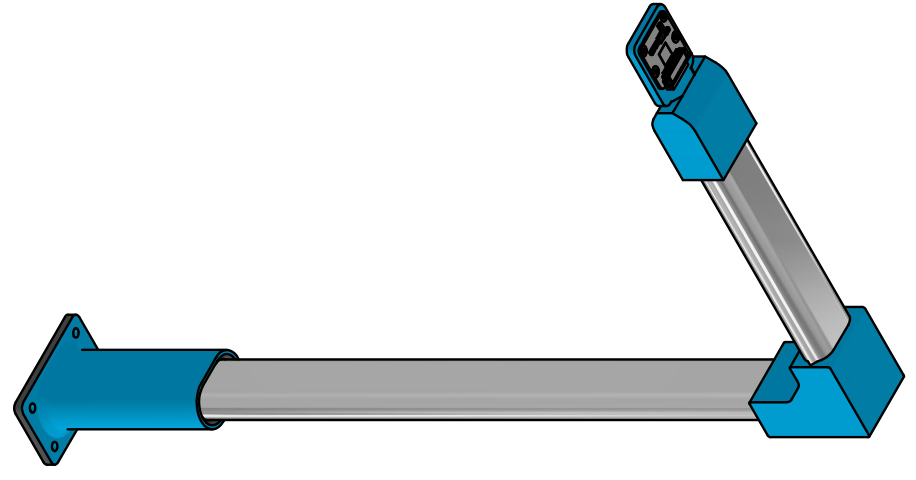
\includegraphics[width=0.55\textwidth]{06disenoConceptual/img/camara/soporteCamaraObsoleto.png}
    \caption{Primera iteración del soporte de cámara mostrando configuración tipo "L" con mástil vertical y viga horizontal en voladizo. Se observa el sistema de uniones por fricción entre tubo ovalado y piezas impresas en FDM.}
    \label{fig:soporteCamaraObsoleto}
\end{figure}

\begin{figure}[H]
    \centering
    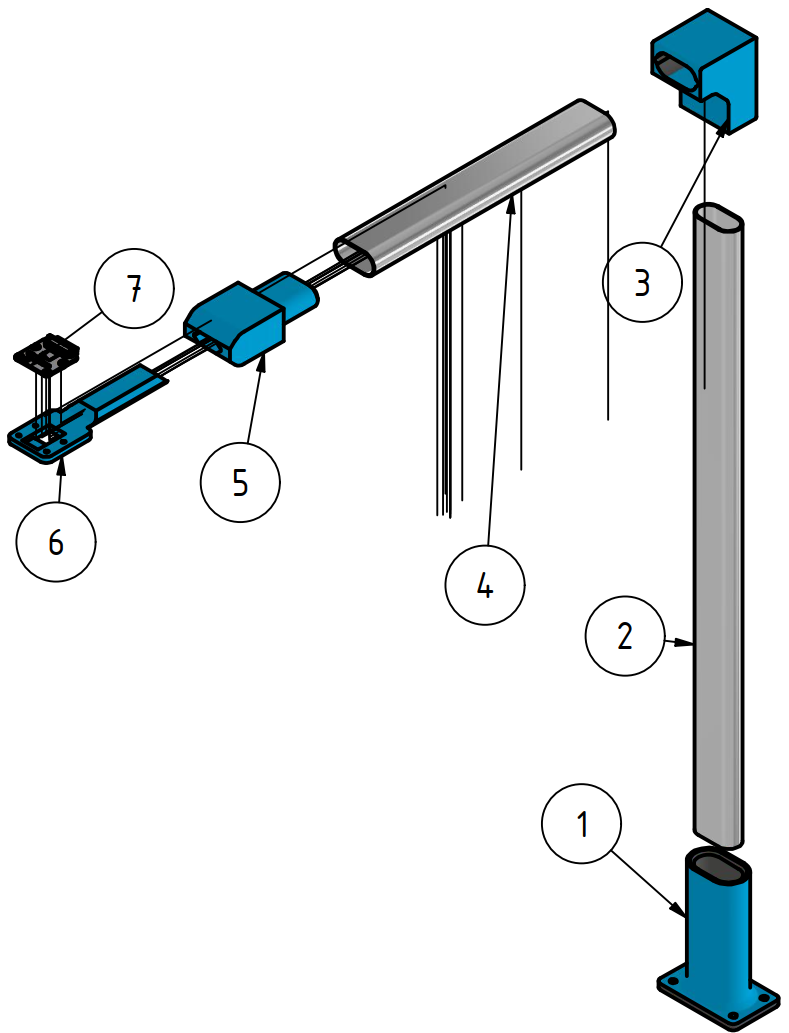
\includegraphics[width=0.6\textwidth]{06disenoConceptual/img/camara/ensambleSoporteCamaraViejo.png}
    \caption{Ensamble explosionado del diseño inicial. (1) Base de mástil con cavidad por fricción, (2) Mástil de tubo ovalado vertical, (3) Codo de 90° con doble cavidad de fricción, (4) Viga horizontal de tubo ovalado, (5) Acople viga-cámara por fricción, (6) Anclaje específico de cámara, (7) Cámara Logitech C270.}
    \label{fig:ensambleSoporteCamaraViejo}
\end{figure}

\begin{table}[H]
\centering
\caption{Componentes del diseño inicial de soporte de cámara}
\label{tab:soporte_camara_v1}
\small
\begin{tabular}{|c|l|c|l|l|}
\hline
\textbf{\#} & \textbf{Componente} & \textbf{Cant.} & \textbf{Fabricación} & \textbf{Material} \\
\hline
1 & Base de mástil & 1 & FDM & ABS/PETG \\
2 & Mástil & 1 & Comercial + corte & Aluminio \\
3 & Codo 90° & 1 & FDM & ABS/PETG \\
4 & Viga & 1 & Comercial + corte & Aluminio \\
5 & Acople viga-cámara & 1 & FDM & ABS/PETG \\
6 & Anclaje de cámara & 1 & FDM & ABS/PETG \\
7 & Cámara & 1 & Comercial & --- \\
\hline
\end{tabular}
\end{table}

\paragraph{Deficiencias Identificadas}

A pesar de la simplicidad conceptual, el diseño por fricción presentó deficiencias críticas durante pruebas de operación extendida:

\begin{itemize}
    \item \textbf{Desgaste de interfaces}: Las cavidades de fricción en piezas FDM (base de mástil, codo, acople de viga) experimentaban deformación plástica progresiva por ciclos de carga/descarga durante vibraciones del manipulador
    
    \item \textbf{Desarrollo de juego mecánico}: Tras 50-100 horas de operación, se observó holgura de 2-5 mm en las uniones, resultando en movimiento de la cámara y pérdida de calibración
    
    \item \textbf{Inestabilidad creciente}: El juego acumulado en múltiples interfaces producía amplificación de vibraciones, comprometiendo la calidad de captura de imágenes
    
    \item \textbf{Ausencia de ajustabilidad}: Una vez instalado, no existía mecanismo para compensar el desgaste sin reemplazar componentes completos
\end{itemize}

Estas deficiencias fundamentaron el desarrollo de una segunda iteración con sistema de fijación mecánica positiva.

\subsubsection{Segunda Iteración: Diseño con Fijación Roscada}

La segunda iteración abandona el concepto de fricción en favor de un sistema de fijación roscada que proporciona rigidez sostenida y ajustabilidad. El diseño conserva modularidad para permitir adaptación a diferentes cámaras.

\paragraph{Versatilidad de Cámaras}

Si bien la selección final fue la Logitech C270, el diseño modular permite intercambio del anclaje de cámara para acomodar sensores alternativos. La Figura \ref{fig:ensamblesCamaras} presenta dos configuraciones: una con cámara ORBBEC Astra y otra con Logitech C270, demostrando la capacidad de adaptación mediante reemplazo del subconjunto de anclaje superior.

\begin{figure}[H]
    \centering
    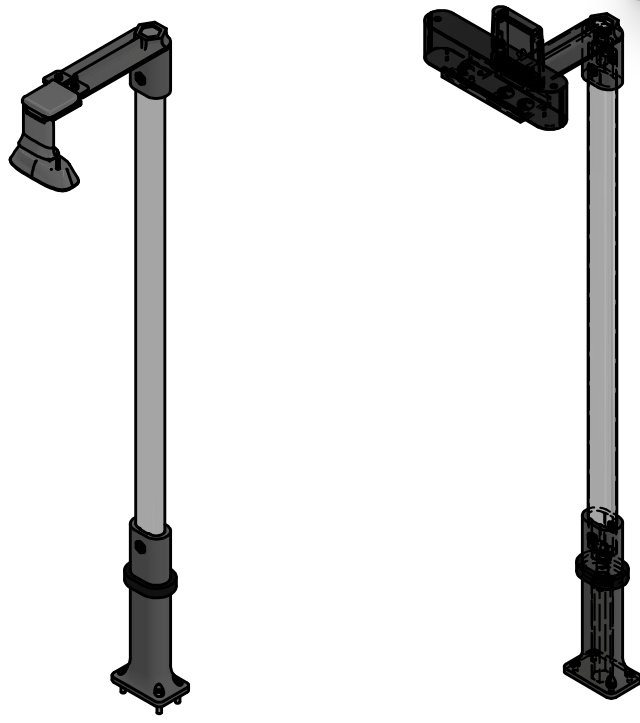
\includegraphics[width=0.7\textwidth]{06disenoConceptual/img/camara/ensamblesCamaras.png}
    \caption{Comparación de configuraciones del soporte con diferentes cámaras. Izquierda: Configuración con cámara ORBBEC Astra RGB-D. Derecha: Configuración con cámara Logitech C270 (seleccionada). Ambas utilizan el mismo mástil y base, intercambiando únicamente el subconjunto de anclaje superior.}
    \label{fig:ensamblesCamaras}
\end{figure}

Esta modularidad preserva inversión en componentes estructurales (mástil, base) si futuras iteraciones del kit requieren sensores con capacidades diferentes.

\paragraph{Determinación de Altura Operativa}

La altura del soporte se determinó empíricamente considerando el campo de visión de las cámaras evaluadas. Se realizaron pruebas de captura a diferentes alturas, identificando que para las cámaras Logitech C270 y ORBBEC Astra (ambas con FOV de aproximadamente 60° diagonal), la altura óptima se encuentra en el rango de 630-710 mm medidos desde la plataforma base hasta el centro del lente.

Esta altura proporciona:
\begin{itemize}
    \item Cobertura completa de la zona de recolección (Ø146 mm)
    \item Visualización de las cuatro zonas de depósito
    \item Margen perimetral de 50-80 mm para compensar desalineamientos
    \item Resolución de 3-4 píxeles/mm sobre objetos de 25 mm × 25 mm
\end{itemize}

\subsubsection{Arquitectura del Conjunto Completo}

El diseño final se estructura en tres subconjuntos principales interconectados mediante tornillería M10 y M4, como se observa en la Figura \ref{fig:ensambleSoporteCamara}.

\begin{figure}[H]
    \centering
    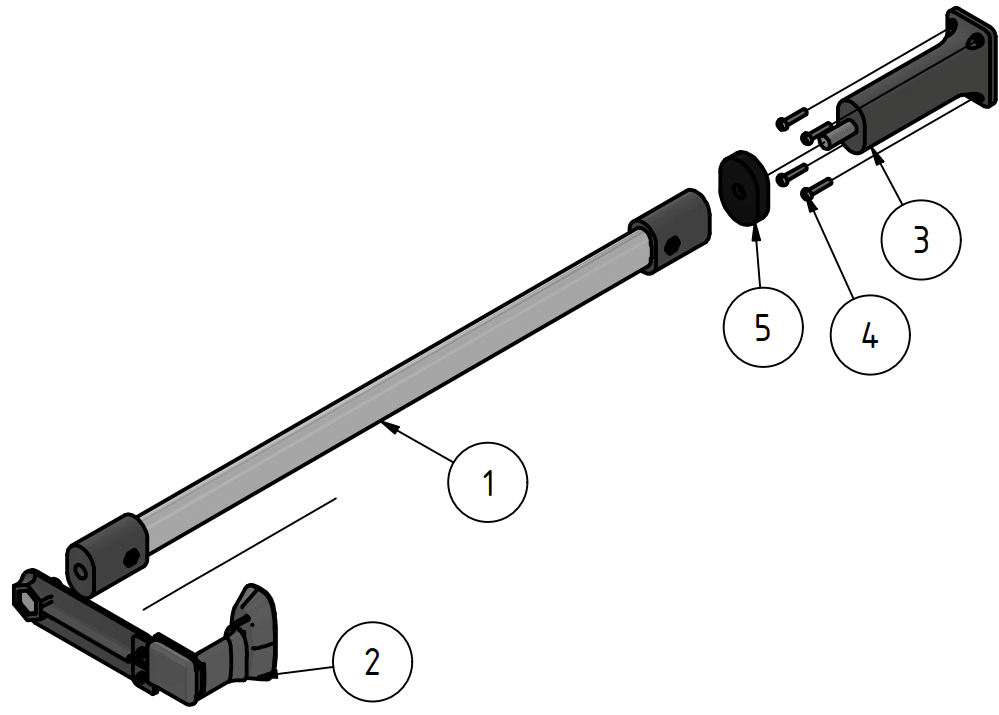
\includegraphics[width=0.8\textwidth]{06disenoConceptual/img/camara/ensambleSoporteCamara.png}
    \caption{Ensamble completo del soporte de cámara versión final. (1) Subconjunto de base de mástil anclado a plataforma, (2) Subconjunto de mástil con encajes roscados en extremos, (3) Subconjunto de soporte superior con viga en voladizo y anclaje de cámara, (4) Tornillos M4 × 20 mm para fijación de base a plataforma (4 unidades), (5) Arandela ovalada de TPU para amortiguación entre mástil y base.}
    \label{fig:ensambleSoporteCamara}
\end{figure}

\begin{table}[H]
\centering
\caption{Componentes principales del soporte de cámara versión final}
\label{tab:soporte_camara_v2}
\small
\begin{tabular}{|c|l|c|l|l|}
\hline
\textbf{\#} & \textbf{Componente} & \textbf{Cant.} & \textbf{Fabricación} & \textbf{Material} \\
\hline
1 & Subconjunto de mástil & 1 & --- & --- \\
2 & Subconjunto soporte superior & 1 & --- & --- \\
3 & Subconjunto base de mástil & 1 & --- & --- \\
4 & Tornillo M4 × 20 mm & 4 & Comercial & Acero \\
5 & Arandela ovalada & 1 & FDM & TPU \\
\hline
\end{tabular}
\end{table}

\paragraph{Función de la Arandela de TPU}

La arandela ovalada de TPU (poliuretano termoplástico) insertada entre el mástil y la base cumple funciones de amortiguación y distribución de carga:

\begin{itemize}
    \item \textbf{Amortiguación de vibraciones}: El TPU, con dureza Shore 95A típica, absorbe vibraciones de alta frecuencia transmitidas desde el manipulador a través de la plataforma
    \item \textbf{Compensación de irregularidades}: La flexibilidad del TPU compensa pequeñas irregularidades de fabricación en las interfaces
    \item \textbf{Distribución de presión}: Previene concentración de esfuerzos en el borde del encaje roscado del mástil
\end{itemize}

\subsubsection{Subconjunto de Mástil}

El mástil constituye el elemento estructural vertical del soporte. La Figura \ref{fig:ensambleMastil} presenta su configuración y la Figura \ref{fig:vistaInternaMastil} revela el mecanismo interno de bloqueo.

\begin{figure}[H]
    \centering
    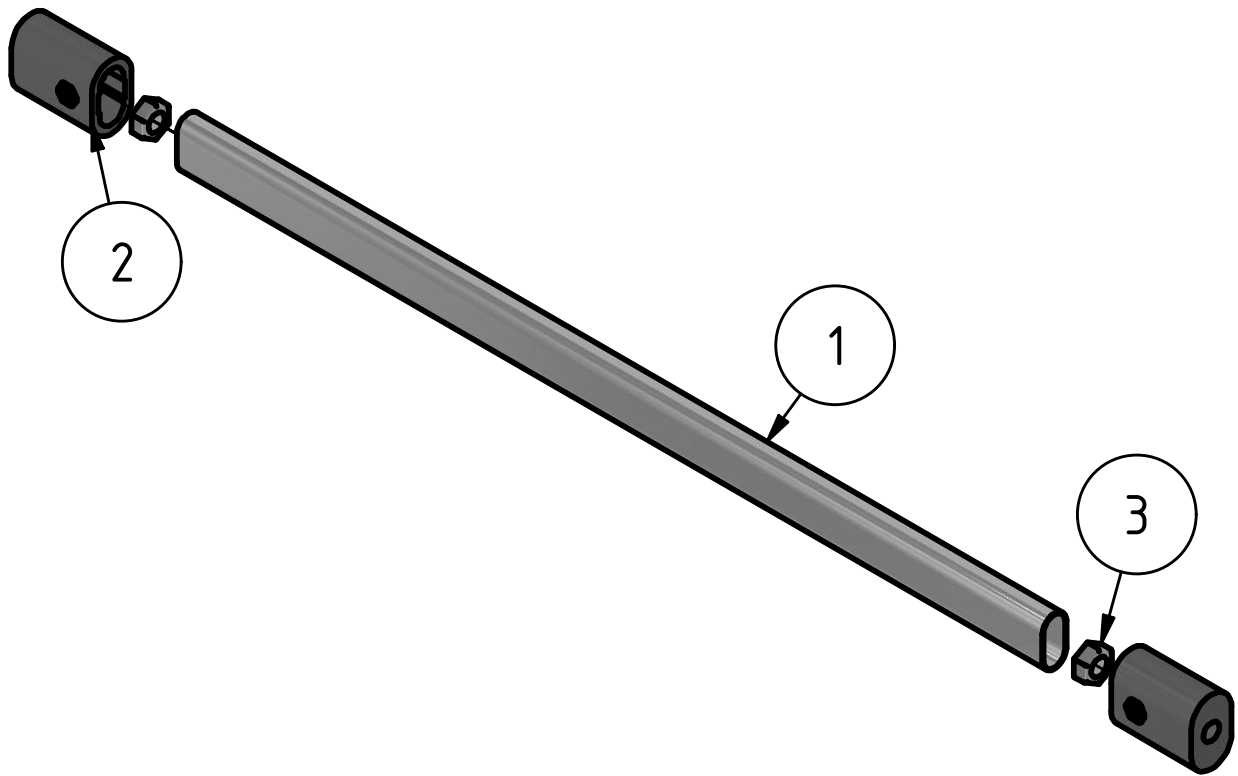
\includegraphics[width=0.6\textwidth]{06disenoConceptual/img/camara/ensambleMastil.png}
    \caption{Ensamble explosionado del subconjunto de mástil. (1) Tubo ovalado de aluminio de 540 mm de longitud, (2) Encajes de tubo a tuerca fabricados en PETG/ABS (2 unidades, superior e inferior), (3) Tuercas M10 alojadas en encajes (2 unidades).}
    \label{fig:ensambleMastil}
\end{figure}

\begin{figure}[H]
    \centering
    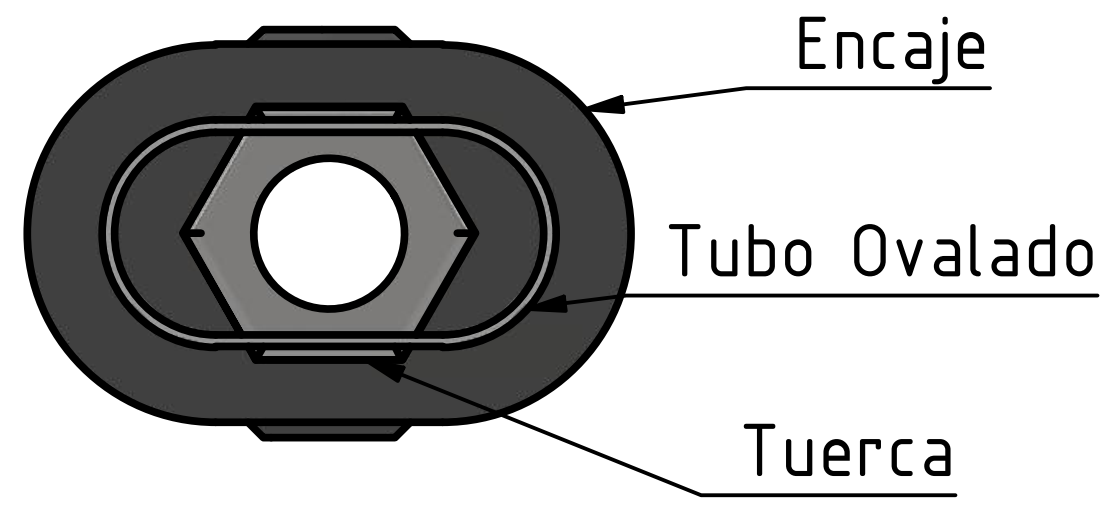
\includegraphics[width=0.5\textwidth]{06disenoConceptual/img/camara/vistaInternaMastil.png}
    \caption{Vista en corte del mecanismo de bloqueo del encaje. El tubo ovalado se inserta en el encaje mediante interferencia o impacto con martillo. Una vez insertado, el perfil ovalado del tubo bloquea la rotación de la tuerca M10 alojada en la cavidad hexagonal del encaje, permitiendo que tornillos externos se enrosquen en la tuerca sin que esta gire.}
    \label{fig:vistaInternaMastil}
\end{figure}

\begin{table}[H]
\centering
\caption{Componentes del subconjunto de mástil}
\label{tab:bom_mastil}
\small
\begin{tabular}{|c|l|c|l|l|}
\hline
\textbf{\#} & \textbf{Componente} & \textbf{Cant.} & \textbf{Fabricación} & \textbf{Material} \\
\hline
1 & Tubo ovalado 540 mm & 1 & Comercial + corte & Aluminio \\
2 & Encaje tubo-tuerca & 2 & FDM & ABS/PETG \\
3 & Tuerca M10 & 2 & Comercial & Acero \\
\hline
\end{tabular}
\end{table}

\paragraph{Restricción Dimensional del Mástil}

La longitud del tubo ovalado (540 mm) se determinó considerando la restricción crítica del contenedor. Durante almacenamiento, el mástil se posiciona diagonalmente dentro del contenedor plástico. Mediante análisis geométrico de la diagonal interna máxima del contenedor (566 mm × 366 mm × altura interna), se estableció que 540 mm es la longitud máxima que permite almacenamiento seguro con margen de 20-30 mm.

Incluyendo los encajes en ambos extremos (18 mm cada uno), la longitud total del subconjunto de mástil es de 576 mm, como se observa en la Figura \ref{fig:largosSoporteCamara}.

\begin{figure}[H]
    \centering
    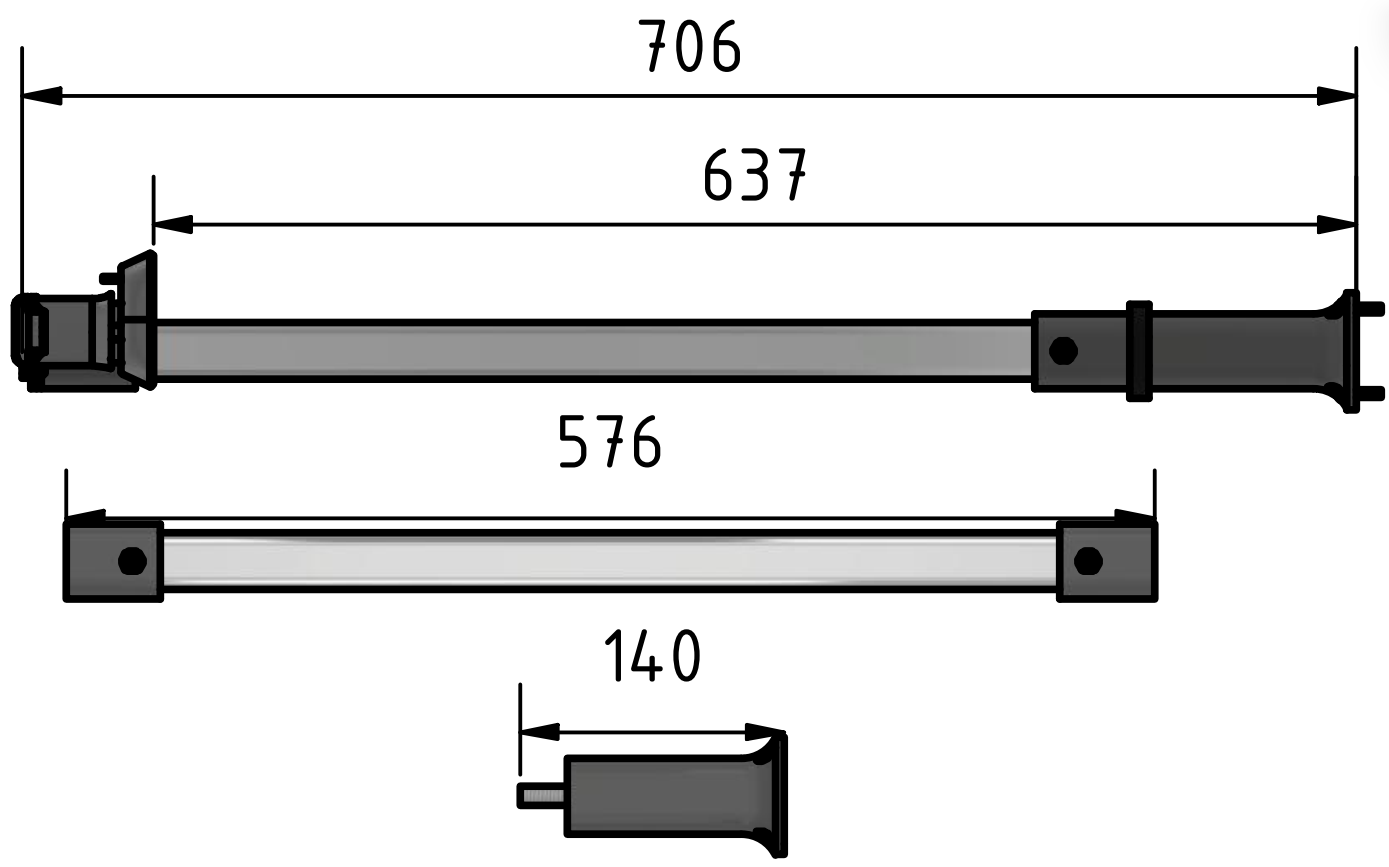
\includegraphics[width=0.85\textwidth]{06disenoConceptual/img/camara/largosSoporteCamara.png}
    \caption{Dimensiones principales de los subconjuntos del soporte de cámara. Superior: Subconjunto completo con longitud total de 706 mm desde base hasta extremo del anclaje de cámara, alcance horizontal de 637 mm desde eje del mástil. Centro: Subconjunto de mástil con longitud total de 576 mm (540 mm de tubo + 2 × 18 mm de encajes). Inferior: Subconjunto de base con altura de 140 mm (altura máxima permitida por contenedor).}
    \label{fig:largosSoporteCamara}
\end{figure}

\paragraph{Mecanismo de Bloqueo Anti-Rotación}

El diseño del encaje aprovecha la geometría ovalada del tubo para crear un sistema de bloqueo automático:

\begin{enumerate}
    \item El encaje se instala en el extremo del tubo mediante interferencia (ajuste apretado) o impacto controlado con martillo de goma
    \item La cavidad interior del encaje tiene geometría ovalada que coincide exactamente con el perfil del tubo
    \item La tuerca M10 se aloja en una cavidad hexagonal dentro del encaje
    \item Cuando el tubo está insertado, su geometría ovalada bloquea completamente la rotación de la tuerca
    \item Tornillos M10 externos pueden enroscarse en la tuerca sin que esta gire, creando unión estructural rígida
\end{enumerate}

Este mecanismo elimina la necesidad de sostener la tuerca con herramientas durante ensamblaje, simplificando el montaje del sistema completo.

\paragraph{Selección de Material PETG/ABS para Encajes}

Los encajes se fabrican en PETG o ABS en lugar de PLA por consideraciones de propiedades mecánicas:

\begin{itemize}
    \item \textbf{Resistencia a impacto}: PETG/ABS absorben energía de impacto durante instalación sin fracturarse (instalación con martillo)
    \item \textbf{Resistencia a fluencia}: Mayor resistencia a deformación plástica bajo carga sostenida que PLA
    \item \textbf{Tenacidad}: Módulo de elasticidad ligeramente inferior al PLA permite pequeñas deformaciones elásticas sin fractura
    \item \textbf{Estabilidad dimensional}: Menor susceptibilidad a cambios dimensionales por absorción de humedad
\end{itemize}

\subsubsection{Subconjunto de Base de Mástil}

La base del mástil proporciona la interfaz entre el tubo vertical y la plataforma del kit. La Figura \ref{fig:ensambleBaseCamara} presenta su configuración interna.

\begin{figure}[H]
    \centering
    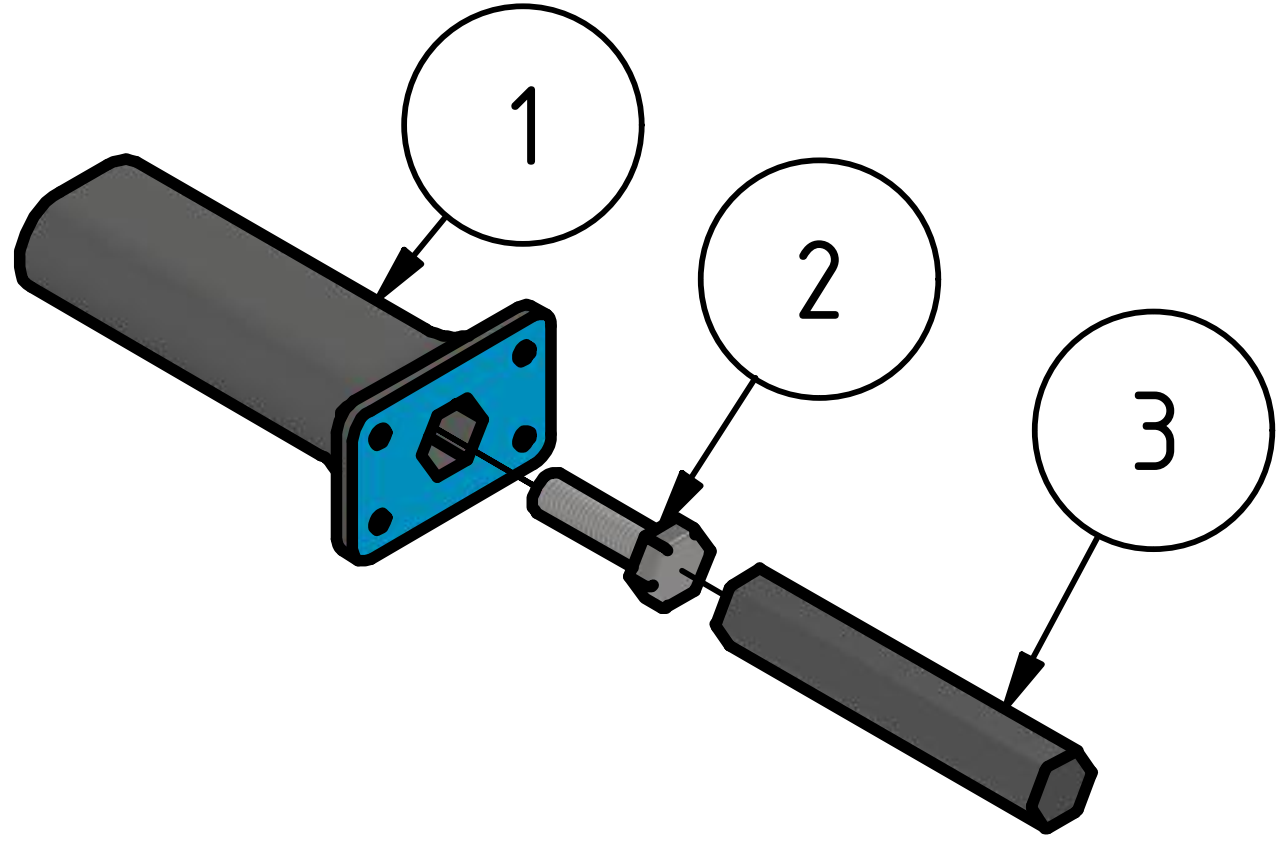
\includegraphics[width=0.55\textwidth]{06disenoConceptual/img/camara/ensambleBaseCamara.png}
    \caption{Ensamble del subconjunto de base de mástil. (1) Tubo ovalado del mástil insertándose en cavidad superior, (2) Tornillo M10 × 35 mm actuando como perno de conexión, (3) Barra hexagonal de refuerzo estructural unida permanentemente con silicona caliente al tornillo y a la base.}
    \label{fig:ensambleBaseCamara}
\end{figure}

\begin{table}[H]
\centering
\caption{Componentes del subconjunto de base de mástil}
\label{tab:bom_base_mastil}
\small
\begin{tabular}{|c|l|c|l|l|}
\hline
\textbf{\#} & \textbf{Componente} & \textbf{Cant.} & \textbf{Fabricación} & \textbf{Material} \\
\hline
1 & Base de mástil & 1 & FDM & ABS/PETG \\
2 & Tornillo M10 × 35 mm & 1 & Comercial & Acero \\
3 & Barra hexagonal de refuerzo & 1 & FDM & ABS/PETG \\
\hline
\end{tabular}
\end{table}

\paragraph{Arquitectura Interna de Refuerzo}

La base incorpora un sistema de refuerzo estructural mediante barra hexagonal interna:

\begin{itemize}
    \item \textbf{Componente}: Barra hexagonal maciza impresa con eje longitudinal paralelo al plano de la cama de impresión
    \item \textbf{Función mecánica}: Resiste cargas de flexión y tensión transmitidas desde el mástil
    \item \textbf{Ventaja de orientación de impresión}: Las capas de impresión quedan orientadas perpendiculares a la dirección de carga principal, aprovechando la mayor resistencia del filamento en dirección paralela a las capas
    \item \textbf{Ensamblaje}: Se une permanentemente al tornillo M10 y a las paredes internas de la base mediante silicona caliente durante fabricación
\end{itemize}

\paragraph{Restricción de Altura por Contenedor}

La altura de la base (140 mm) está limitada por la altura interna del contenedor plástico. Si la base excediera esta dimensión, el contenedor no podría cerrarse correctamente. La Figura \ref{fig:vistaInternaKitBaseMastil} ilustra esta restricción crítica de diseño.

\begin{figure}[H]
    \centering
    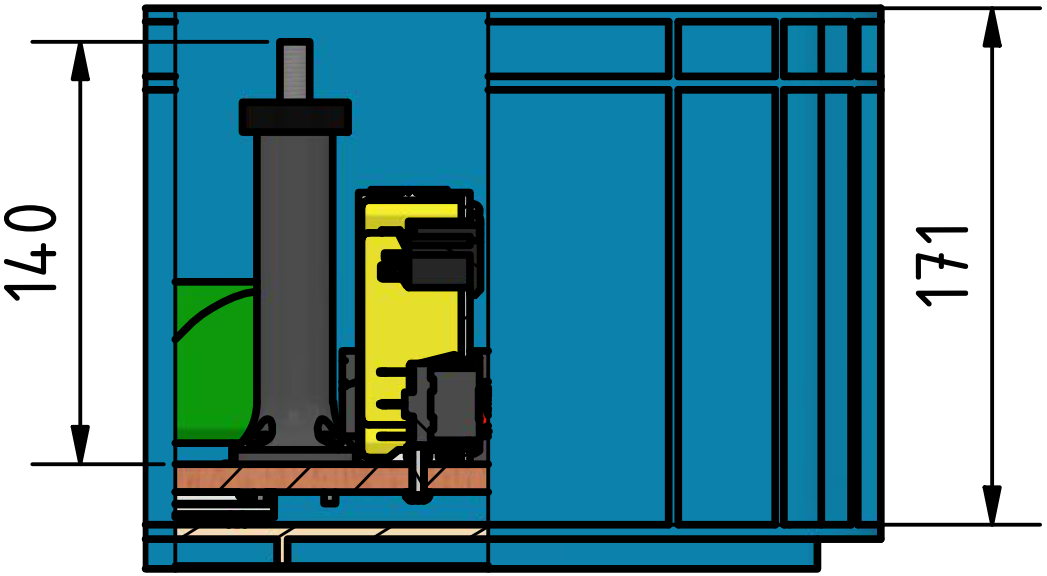
\includegraphics[width=0.75\textwidth]{06disenoConceptual/img/camara/vistaInternaKitBaseMastil.png}
    \caption{Vista en corte del interior del contenedor con base de mástil instalada. Altura interna del contenedor: 171 mm. Altura de la base: 140 mm. La base (verde) no excede la altura interna, permitiendo cierre correcto de la tapa. Se observa la arandela de TPU (naranja) entre base y plataforma.}
    \label{fig:vistaInternaKitBaseMastil}
\end{figure}

\paragraph{Consideraciones de Orientación de Impresión}

La base del mástil se imprime con su eje longitudinal perpendicular a la cama de impresión (vertical). Esta orientación:

\begin{itemize}
    \item \textbf{Ventaja geométrica}: Minimiza soportes y facilita extracción de la pieza
    \item \textbf{Desventaja mecánica}: Las capas quedan paralelas a la dirección de carga de tensión, reduciendo resistencia en aproximadamente 30-40\% respecto a orientación horizontal
    \item \textbf{Compensación}: La barra hexagonal interna, impresa horizontalmente, compensa esta debilidad proporcionando el 60-70\% de la resistencia estructural del conjunto
\end{itemize}

\subsubsection{Subconjunto de Soporte Superior}

El soporte superior constituye el elemento en voladizo que posiciona la cámara sobre el centro de la zona de trabajo. La Figura \ref{fig:soporteSuperiorC270} presenta su configuración modular.

\begin{figure}[H]
    \centering
    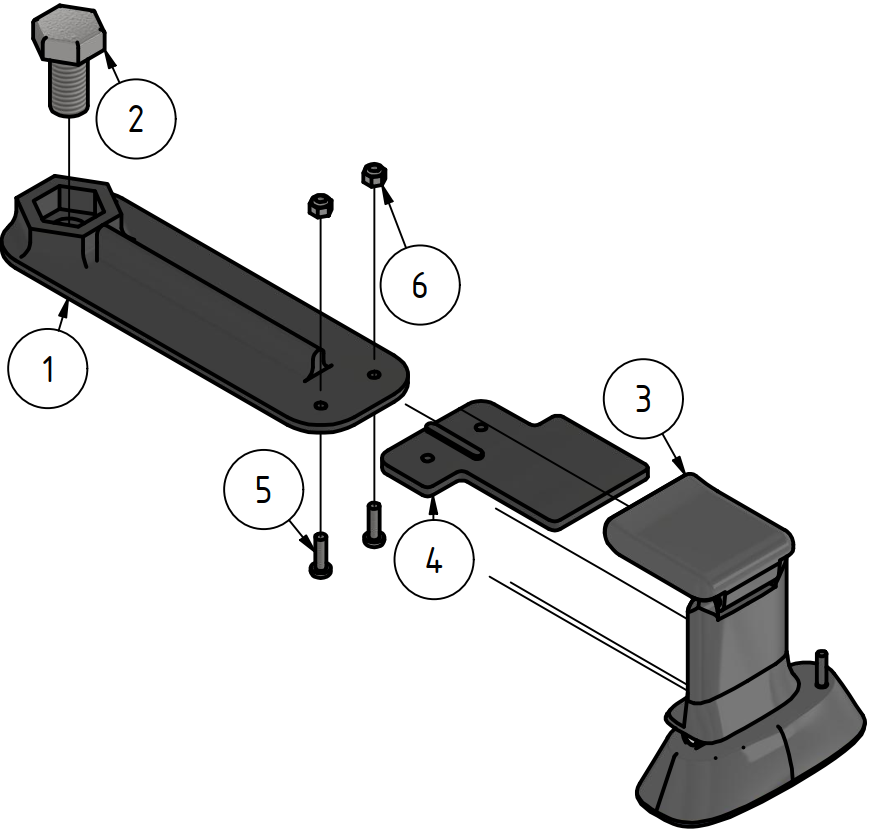
\includegraphics[width=0.75\textwidth]{06disenoConceptual/img/camara/soporteSuperiorC270.png}
    \caption{Ensamble del subconjunto de soporte superior para cámara Logitech C270. (1) Viga de soporte fabricada en PETG/ABS, (2) Tornillo M10 × 20 mm unido permanentemente a la viga con silicona, que se enrosca en tuerca del extremo superior del mástil, (3) Cámara Logitech C270, (4) Anclaje modular específico de cámara, (5) Tornillos M3 × 10 mm (2 unidades), (6) Tuercas de seguridad M3 (2 unidades).}
    \label{fig:soporteSuperiorC270}
\end{figure}

\begin{table}[H]
\centering
\caption{Componentes del subconjunto de soporte superior}
\label{tab:bom_soporte_superior}
\small
\begin{tabular}{|c|l|c|l|l|}
\hline
\textbf{\#} & \textbf{Componente} & \textbf{Cant.} & \textbf{Fabricación} & \textbf{Material} \\
\hline
1 & Viga de soporte de cámara & 1 & FDM & ABS/PETG \\
2 & Tornillo M10 × 20 mm & 1 & Comercial & Acero \\
3 & Cámara Logitech C270 & 1 & Comercial & --- \\
4 & Anclaje de cámara a viga & 1 & FDM & ABS/PETG \\
5 & Tornillo M3 × 10 mm & 2 & Comercial & Acero \\
6 & Tuerca de seguridad M3 & 2 & Comercial & Acero \\
\hline
\end{tabular}
\end{table}

\paragraph{Conexión Viga-Mástil}

La viga se une al mástil mediante tornillo M10 × 20 mm que se enrosca en la tuerca cautiva del encaje superior del mástil. El tornillo se fija permanentemente a la viga mediante silicona caliente aplicada en una cavidad interna, garantizando que:

\begin{itemize}
    \item El tornillo no se afloje por vibraciones durante operación
    \item La unión viga-mástil pueda ajustarse o removerse desenroscando el tornillo sin que este se separe de la viga
    \item La orientación angular de la viga respecto al mástil pueda ajustarse durante instalación inicial
\end{itemize}

\paragraph{Modularidad del Anclaje de Cámara}

El anclaje de cámara se diseña específicamente para cada modelo de cámara contemplado. Para la Logitech C270, el anclaje:

\begin{itemize}
    \item Abraza el cuerpo cilíndrico de la cámara con geometría complementaria
    \item Se fija a la viga mediante dos tornillos M3 × 10 mm con tuercas de seguridad
    \item Permite ajuste de inclinación (±10°) antes de apriete final
    \item Posiciona el lente de la cámara alineado con el centro de la zona de recolección
\end{itemize}

Para cámaras alternativas (ORBBEC Astra, Intel RealSense), solo requiere reemplazo del anclaje específico, reutilizando viga, mástil y base.

\paragraph{Alineación Óptica}

El diseño del anclaje garantiza que el centro óptico del lente de la cámara esté alineado con el eje vertical que pasa por el centro de la zona de recolección (Ø146 mm, blanca). La Figura \ref{fig:vistaSuperiorCamaraKit} demuestra esta alineación en vista superior.

\begin{figure}[H]
    \centering
    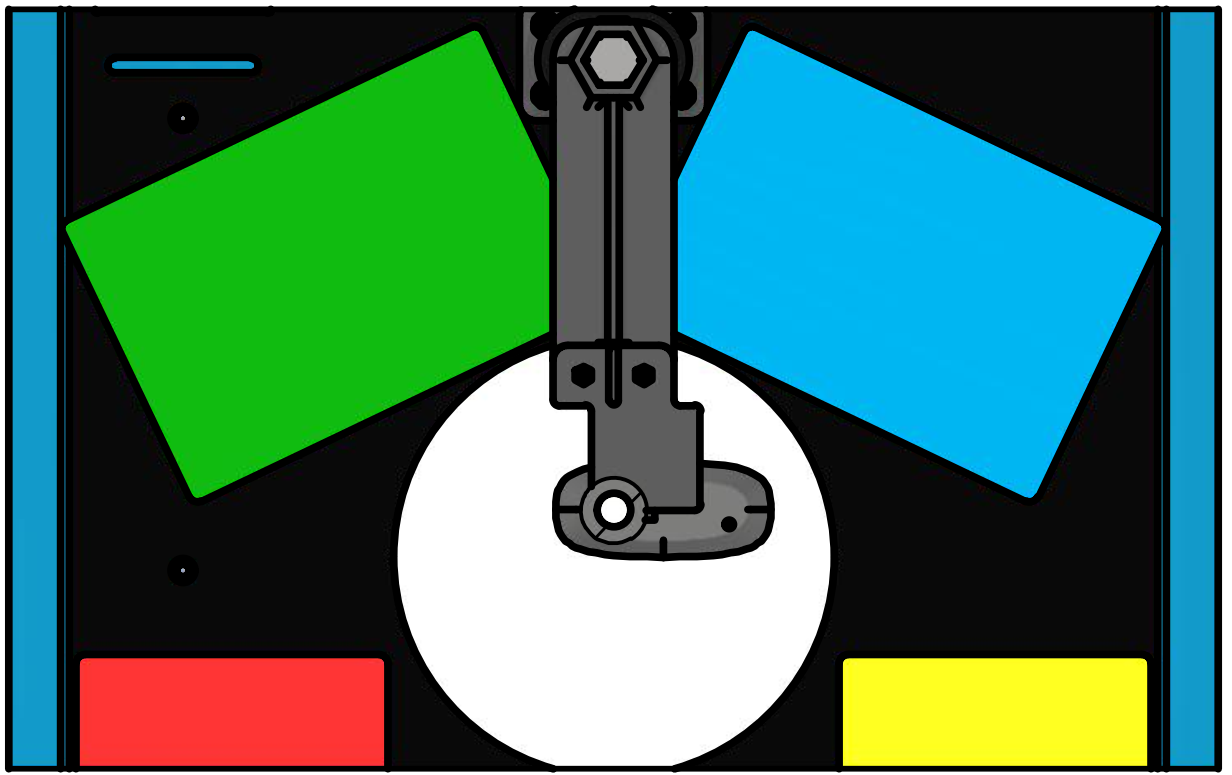
\includegraphics[width=0.8\textwidth]{06disenoConceptual/img/camara/vistaSuperiorCamaraKit.png}
    \caption{Vista superior del kit mostrando alineación del eje óptico de la cámara. El centro del lente (indicado por proyección vertical) coincide con el centro geométrico de la zona de recolección (blanca, Ø146 mm). Esta alineación minimiza distorsión perspectiva en los bordes de la zona de trabajo y simplifica la calibración del sistema de visión.}
    \label{fig:vistaSuperiorCamaraKit}
\end{figure}

Esta alineación centrada proporciona:
\begin{itemize}
    \item Distorsión perspectiva simétrica respecto al centro de la imagen
    \item Simplificación de transformaciones pixel-a-mundo (matriz homográfica con punto principal centrado)
    \item Cobertura equidistante de zonas de depósito desde el centro óptico
    \item Reducción de oclusiones en bordes de la zona de recolección
\end{itemize}

\subsection{Conclusión del Diseño del Soporte}

El diseño final del soporte de cámara representa una evolución significativa respecto a la iteración inicial, incorporando lecciones aprendidas sobre desgaste de interfaces y estabilidad dimensional. El sistema de fijación roscada M10 proporciona rigidez sostenida, la arquitectura modular permite adaptación a diferentes sensores, y las restricciones dimensionales del contenedor se satisfacen mediante optimización de alturas y longitudes. El resultado es un soporte robusto, ajustable y versátil que garantiza posicionamiento estable del sensor visual durante operación extendida del kit educativo.